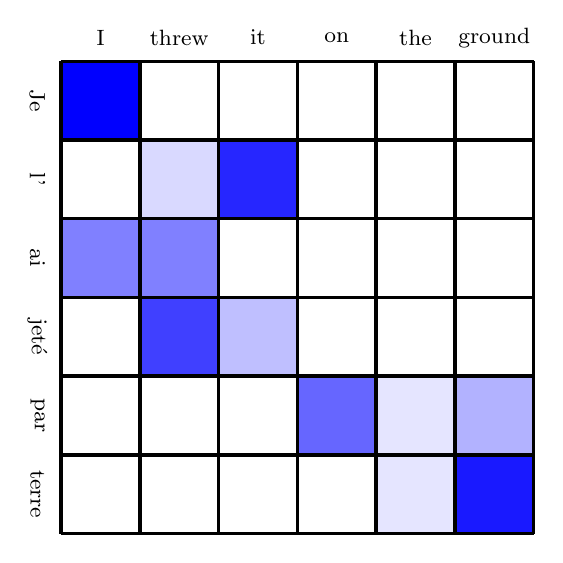
\begin{tikzpicture}[word/.style={font=\footnotesize, inner sep=0pt}]
    \foreach \i/\word in {0/I, 1/threw, 2/it, 3/on, 4/the, 5/ground} {
        \node at (\i + 0.5, 0.3) [word] {\word};
    }

    \foreach \i/\word in {0/Je, 1/l', 2/ai, 3/jet\'e, 4/par, 5/terre} {
        \node at (-0.3, -\i - 0.5) [word, rotate=270] {\word};
    }

    % Je
    \fill [blue] (0, 0) rectangle (1, -1);

    % l’
    \fill [blue!15] (1, -1) rectangle (2, -2);
    \fill [blue!85] (2, -1) rectangle (3, -2);

    % ai
    \fill [blue!50] (0, -2) rectangle (1, -3);
    \fill [blue!50] (1, -2) rectangle (2, -3);

    % jete
    \fill [blue!75] (1, -3) rectangle (2, -4);
    \fill [blue!25] (2, -3) rectangle (3, -4);

    % par
    \fill [blue!60] (3, -4) rectangle (4, -5);
    \fill [blue!10] (4, -4) rectangle (5, -5);
    \fill [blue!30] (5, -4) rectangle (6, -5);

    % terre
    \fill [blue!10] (4, -5) rectangle (5, -6);
    \fill [blue!90] (5, -5) rectangle (6, -6);

    \draw [very thick] (0, 0) grid (6, -6);
\end{tikzpicture}
%%% Local Variables:
%%% mode: latex
%%% TeX-master: "../rnn"
%%% End:
